\documentclass[12pt,a4paper]{article}
\usepackage{amsmath, amssymb} % Math Packages
\usepackage{geometry}
\usepackage[hidelinks]{hyperref} % Clickable links
\usepackage{graphicx, float} % Image Packages
\graphicspath{{/home/tyler/Obsidian Vaults/Notes/Config}} % Path to image folder
\geometry{margin=2cm}
\setlength{\parindent}{0pt} % No indentation
\usepackage[table]{xcolor}
\usepackage{tabularx}
\usepackage{array}
\usepackage[none]{hyphenat} % Disable Hypens splitting words across lines

\begin{document}
\begin{center}
\textbf{\LARGE ENG306\\[6pt]
Power Electronics}\\[10pt]
\textbf{\large Lab 2\\[4pt]
Baley Eccles - 652137\\
Tyler Robards - 651790}\\
\end{center}

\tableofcontents
\newpage
\section{Introduction}
NOTE: Mention We had issues with saving data from the scope
\section{Diode Rectifiers}
\subsection{Half-Wave Rectifier with Resistive Load}
\textit{Plot(using data saved from the oscilloscope) or insert screenshots or sketch by hand, 
waveforms for $v_s$, $v_o$, $i_o$ and $v_D$ using the same time-scale x axis (so that they can be
easily compared – including diode voltage), and discuss your observations briefly.}\\


\textit{From your waveform measurements using oscilloscope, compare the dc output current 
and voltage against digital multimeter measurements and also against values determined by applying 
theoretical relationships for this rectifier. Present the different measurements and calculated 
values in table form, commenting on your observations.}\\


\subsection{Full-Wave Rectifier with Resistive and Inductive Load}
\textit{Why was it necessary to measure the rectifier supply voltage waveform using the oscilloscope
probes on the second of the two secondary windings or using two probes and the maths function?
Describe what you think would happen if probes were still placed across the first winding (i.e.
between points 1 and 2 on the circuit).}\\

\textit{For the resistive load only set up, plot (using data saved from the oscilloscope) or insert screenshots
or sketch by hand, waveforms for $v_s$, $v_o$, $i_o$ using the same time-scale x axis, and discuss your
observations.}\\

\textit{Again for the resistive load only, from your waveform measurements using oscilloscope, compare
the dc output current and voltage against digital multimeter measurements and also against values
determined by applying theoretical relationships for this rectifier. Present the different measurements
and calculated values in table form, commenting on your observations.}\\

\textit{For the resistive and inductive load, plot (using data saved from the oscilloscope) or insert
screenshots or sketch by hand, waveforms for $v_s$, $v_o$, $i_o$ and $v_D$ for the two diodes measured, using
the same time-scale x axis (so that they can be easily compared – including diode voltage), and
discuss your observations, including comparing against what was observed for resistive only load}\\

\textit{Present your measured average (dc) and rms values of output voltage and current (for RL load).
How do they compare to the values measured for the resistive load only and why?}\\

\textit{By considering losses in the four diodes, estimate your overall rectifier circuit efficiency. Note: there
are a few approaches you can take here, some which may require you to think about and perform
some more measurements in the lab.}\\
\subsection{Full-Wave Rectifier with Capactive Output Filter and Resistive Load}
\textit{Tabulate, to allow for easy comparison, your measured dc output voltage and peak-to-peak ripple for each of the three capacitors values}\\\\

\begin{center}
	\begin{tabular}{|c|c|c|}
		\hline
		\centering\textbf{Capacitor Size} & \centering\textbf{DC Output Voltage $V_{dc}$} &\centering\textbf{Peak-to-Peak Ripple $V_{pp}$}\tabularnewline 
		\hline
		$470 F$ & $2.1V$ & $7V$ \\
		\hline
		$1000 F$ & $1.2V$ & $4.4V$\\
		\hline
		$2000 F$ & $0.5V$ & $2.35V$\\
		\hline
	\end{tabular}
\end{center}

\textit{Carefully plot (using data saved from the oscilloscope) or sketch by hand on one graph the output voltage waveform observed for each of the three capacitor values. Comment on how and why the
waveforms and measurements differ with changing capacitor value.}\\\\

TODO: Comments on the plots
\begin{figure}[H]
        \centering
	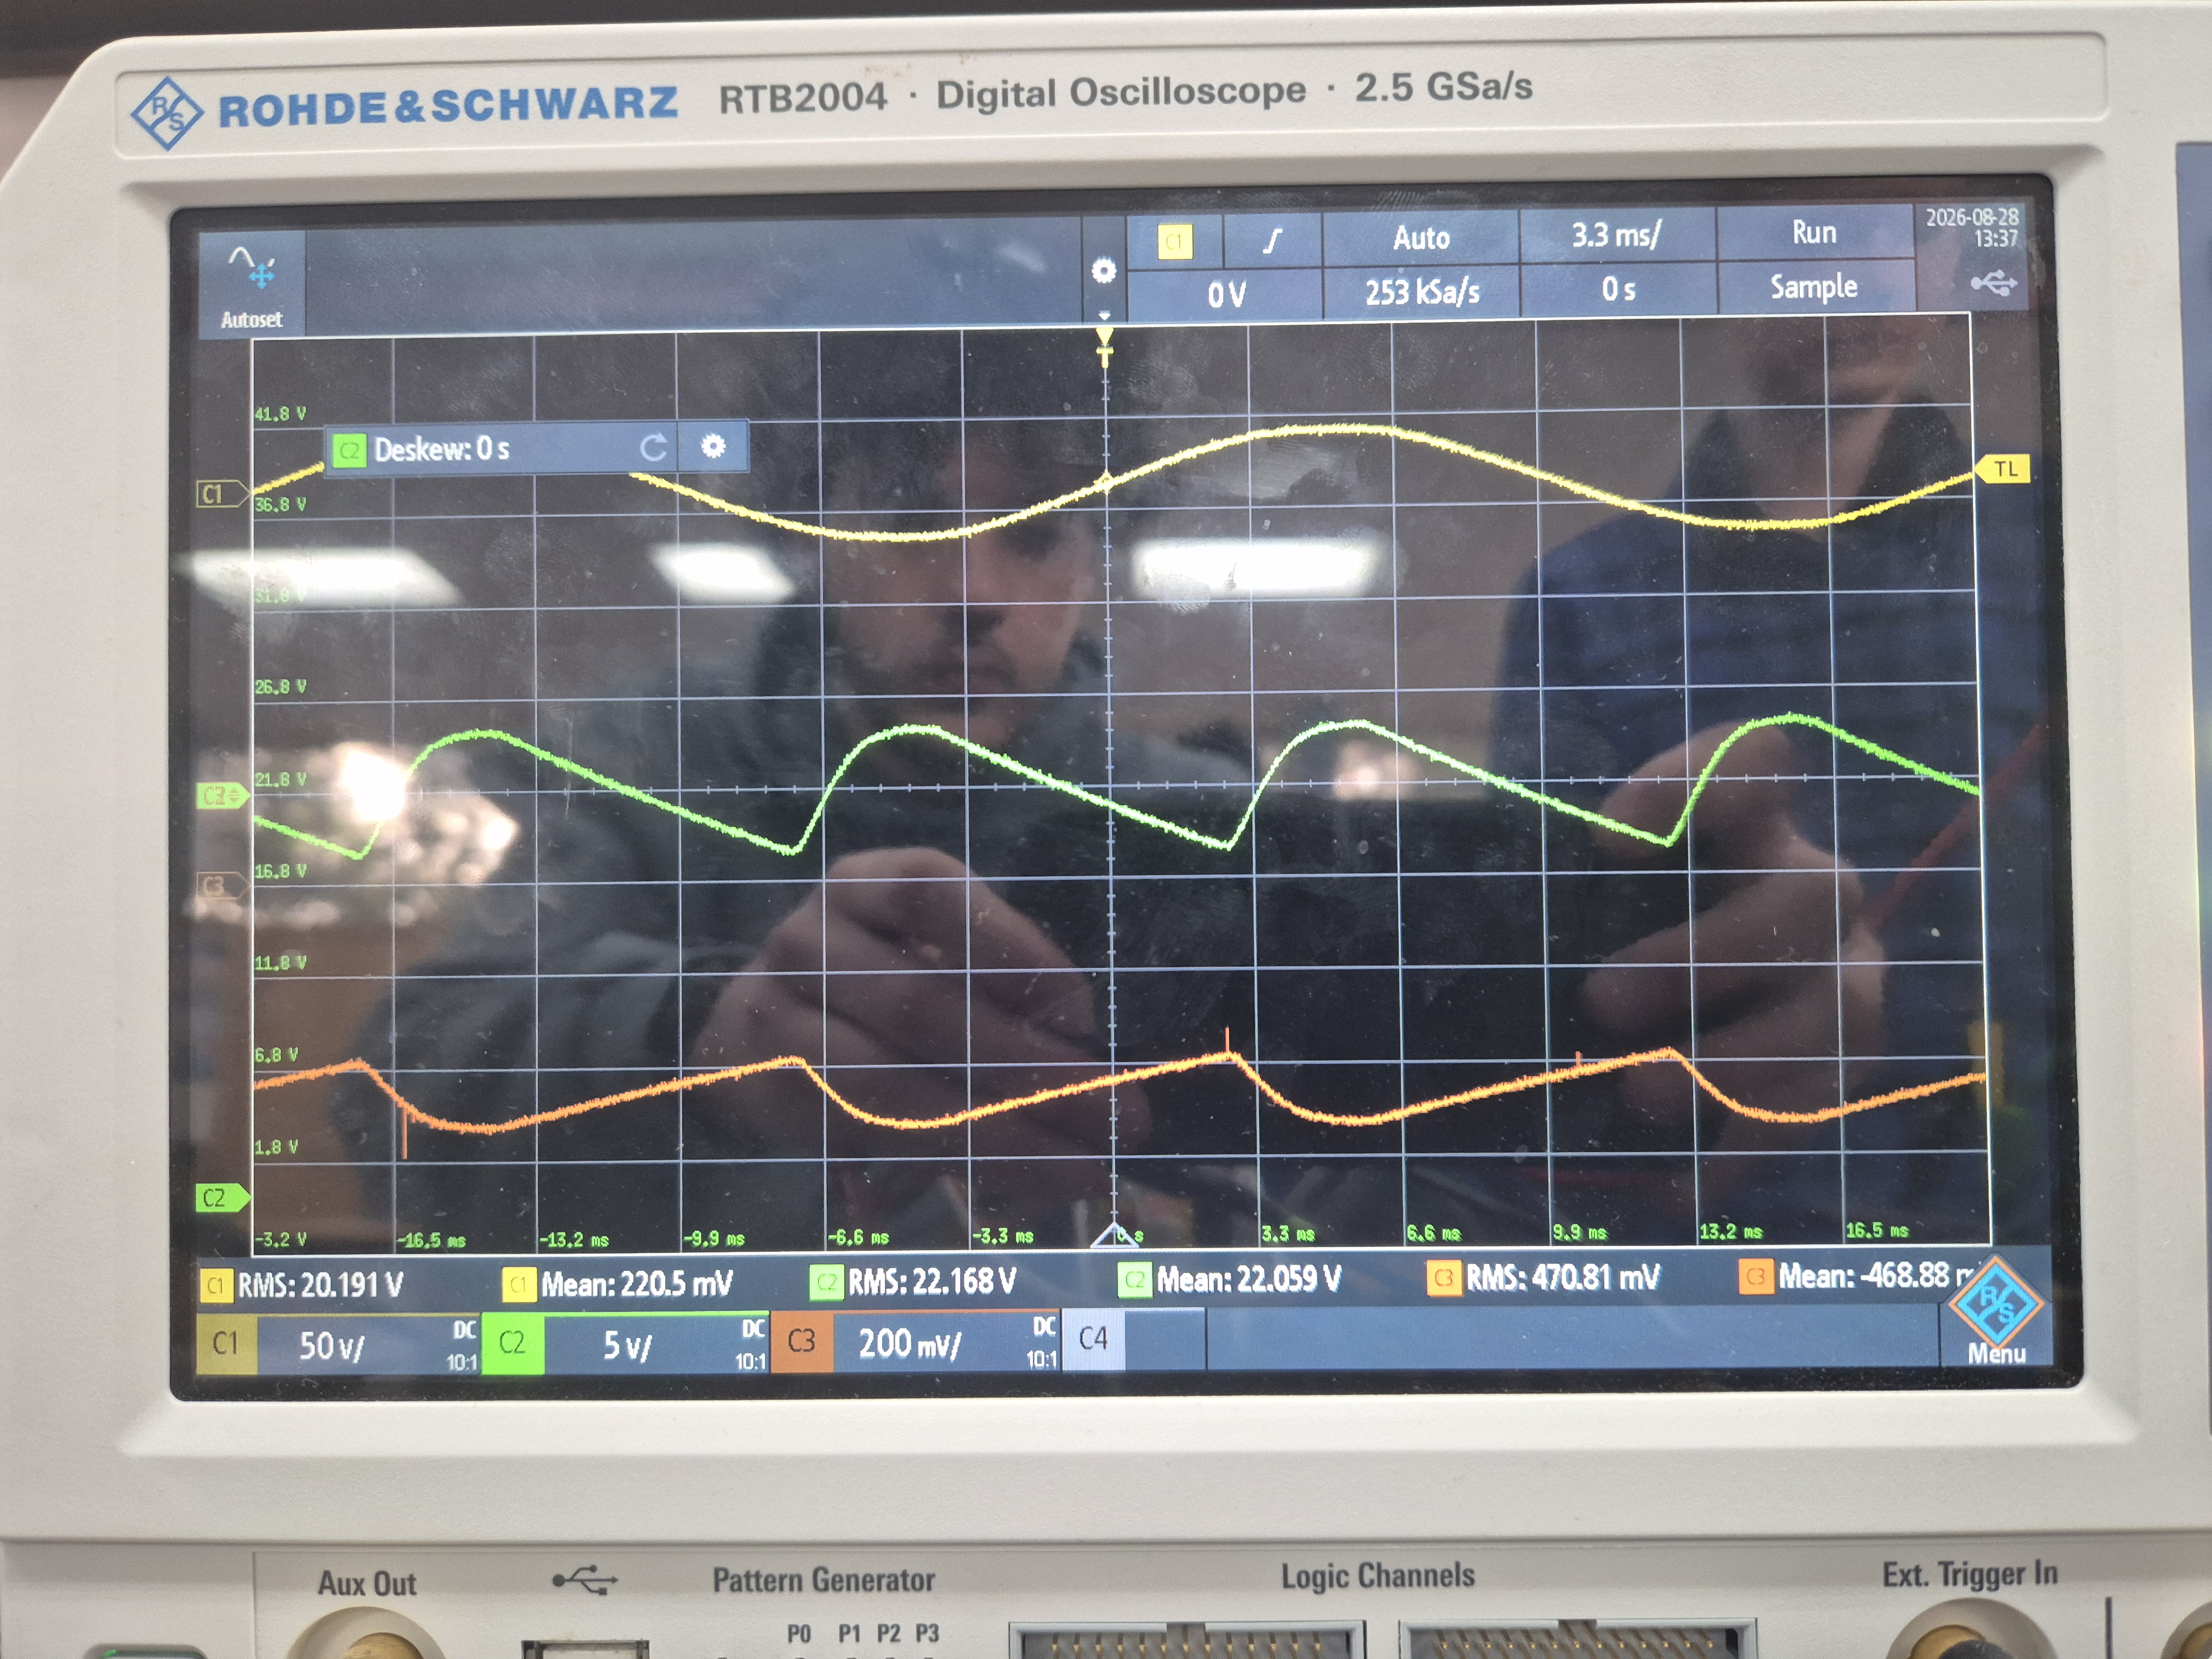
\includegraphics[width=0.7\columnwidth]{Images/20250828_134829.jpg}
	\caption{$470F$ Capacitor Plot}
	\label{fig:470F Cap Plot}
\end{figure}
\begin{figure}[H]
        \centering
	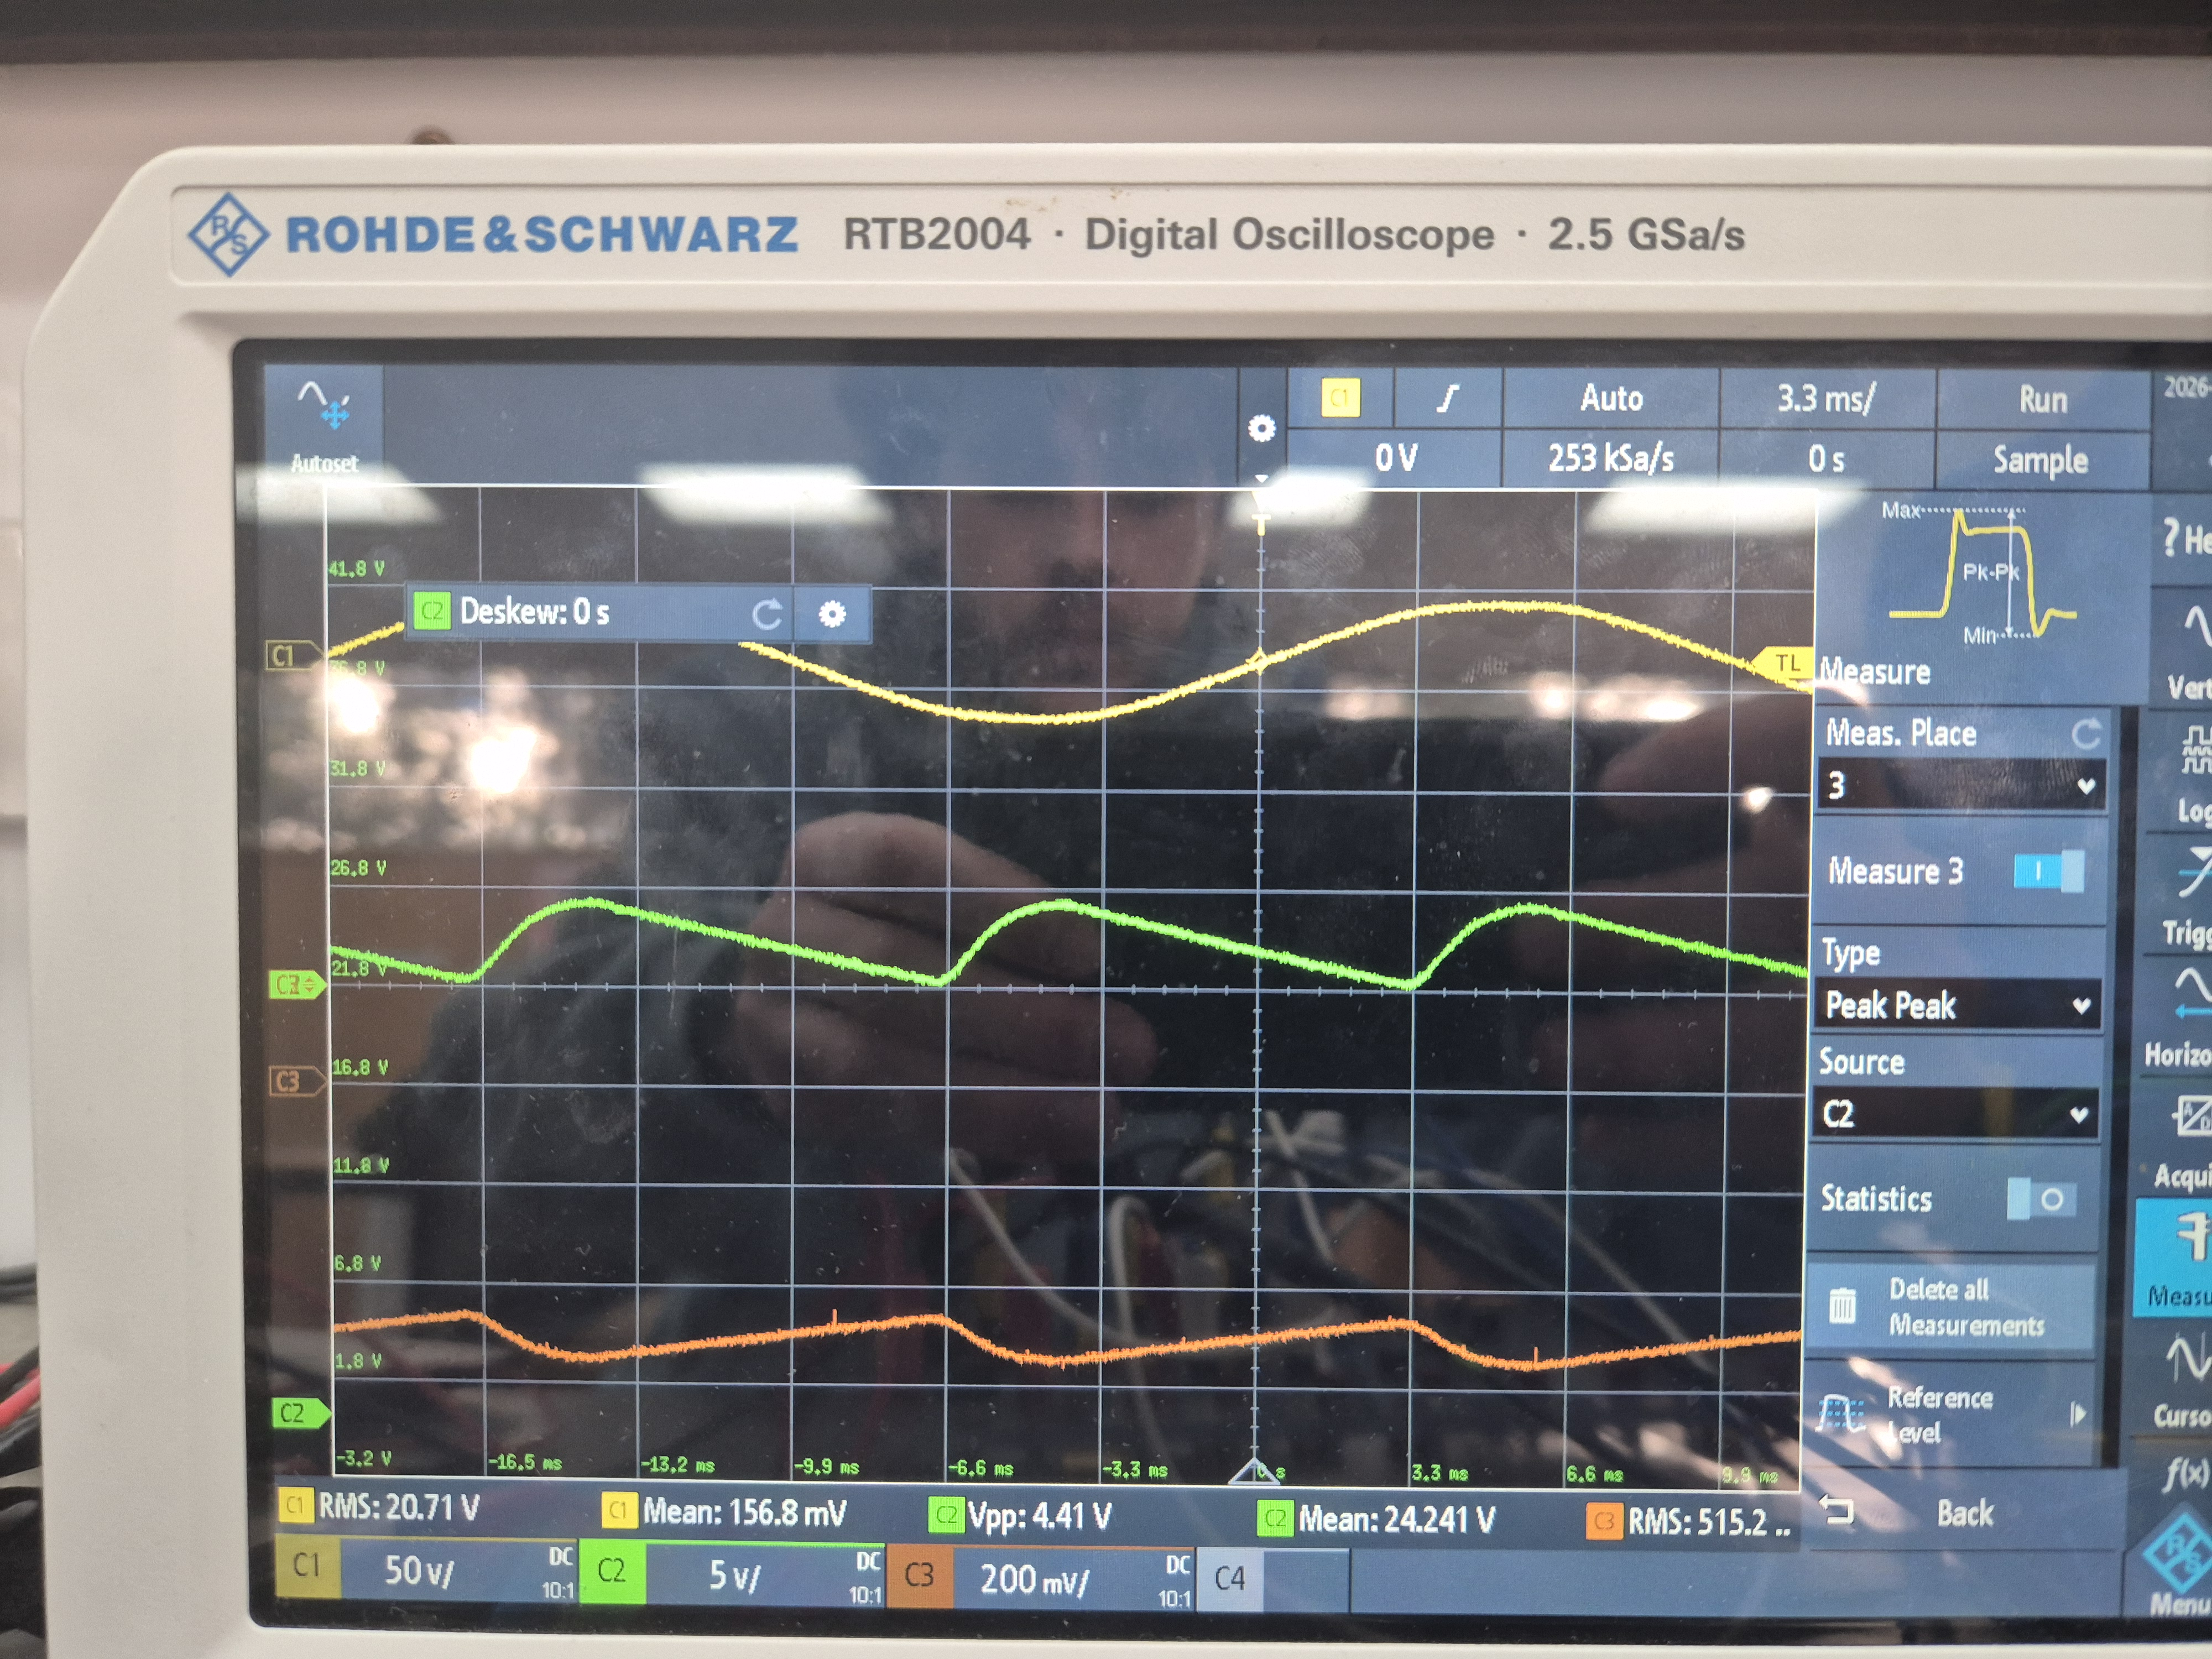
\includegraphics[width=0.7\columnwidth]{Images/20250828_135102.jpg}
	\caption{$1000$ Capacitor Plot}
	\label{fig:1000F Cap Plot}
\end{figure}
\begin{figure}[H]
        \centering
	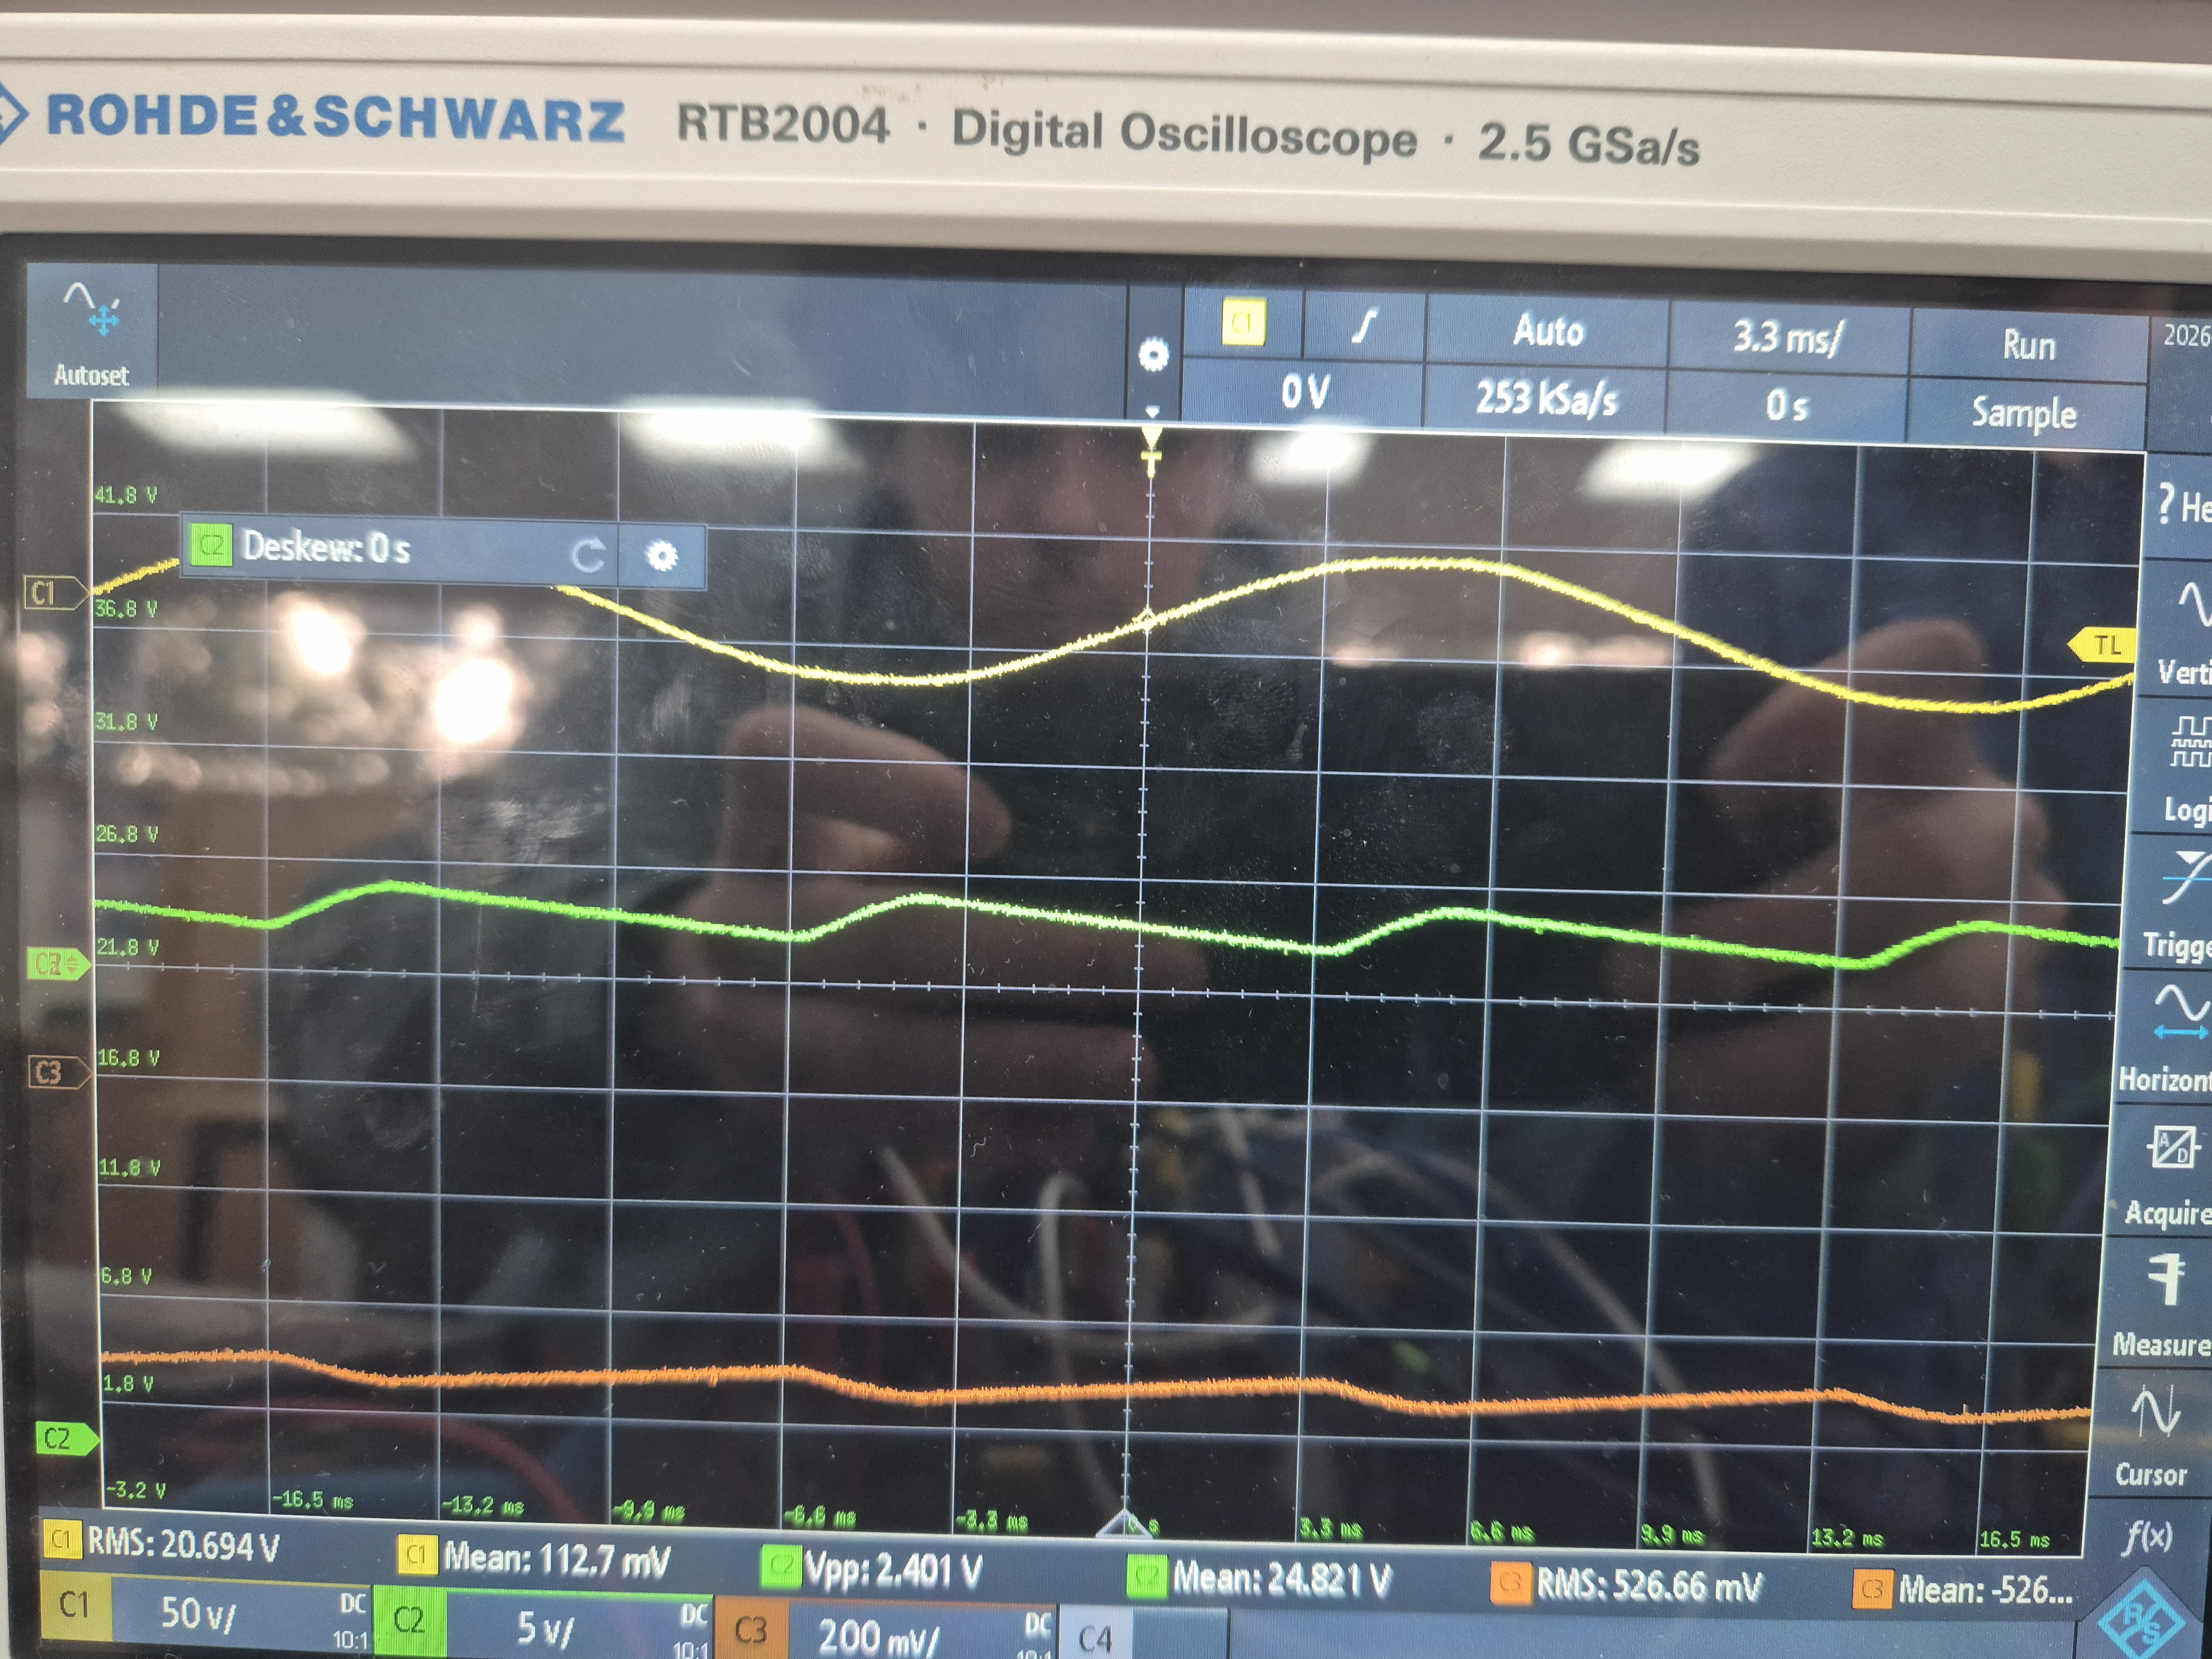
\includegraphics[width=0.7\columnwidth]{Images/20250828_135318.jpg}
	\caption{$2000$ Capacitor Plot}
	\label{fig:2000F Cap Plot}
\end{figure}


\textit{Develop an approximate expression for percentage peak-to-peak ripple as a function of R, C and
frequency $f$, stating carefully any assumptions. How do your calculated values, using your derived
expression, compare to your measurements?}\\

\textit{How would you expect the value of the capacitor to impact upon supply current waveform, in
particular on the harmonic content? Describe why you expect this?
(Note: if you have time you may wish to think of a way to measure and display the Fourier
components of supply current for your circuit, thus gaining extra insight}\\
\section{Thyristor Controller Rectifiers}
\subsection{Semi-Converter with Resitive and Inductive Load}
\begin{center}
\begin{tabular}{|p{3cm}|p{2.5cm}|p{2.5cm}|p{2.5cm}|}
\hline
\centering\textbf{Firing angle} &
\multicolumn{2}{c|}{\textbf{Digital multimeter}} &
\centering\textbf{Calculated} \tabularnewline
\hline
\centering$\alpha$ & \centering$V_o$ & \centering$I_o$ & \centering$V_o$ \tabularnewline
\hline
0 & 0 & 0 & \\ \hline
20 & 0.8 & 0.8 & \\ \hline
45 & 3.4 & 20 & \\ \hline
60 & 5.6 & 63 & \\ \hline
90 & 9.7 & 159 & \\ \hline
100 & 10.2 & 184 & \\ \hline
120 & 10.9 & 247 & \\ \hline
140 & 10.6 & 285 & \\ \hline
160 & 9.5 & 317 & \\ \hline
180 & 8.8 & 333 & \\ \hline
\end{tabular}
\end{center}\\
\textit{Detail the way you connected your oscilloscope probes and configured the oscilloscope to record simultaneously the source voltage, trigger signal, output voltage and current waveforms.}\\\\

The common ground is at $+V_o$ to allow for common measurments. Channel 1 measures the source voltage using the secondary transformer winding. This is acceplatble as it is electrlcally isolated from the remainder of the circuit so multiple grounds cannot cause a short circuit. Channel 2 measure the output voltage, with it's positive probe placed at $-V_o$. Channel 3 measures $I_o$, with it's probe placed between the $1\Omega$ and $47\Omega$ resistors. Measuring the voltage over the $1\Omega$ resistor is equivalent to measuring current as $V=IR$. Channel 4 measures the positive trigger input of $T_1$. \\\\ 

\textit{Include plot from oscilloscope of all waveforms for a firing angle of 45°.}\\\\

TODO: Add plot.\\\\

\textit{Comment on the observed waveforms and on how they changed with firing angle, describing your observations by considering theory of the circuit operation.}\\\\


\textit{From your measured data, create a plot of dc output voltage vs firing angle. Also include in the plot a curve based on theoretical considerations for this circuit. Discuss your findings}\\\\

\textit{Based on your observation, at what firing angle did you observe there to first be a boundary between continuous and discontinuous conduction (of current in the load). Compare to what you might expect from a theoretical view point?}\\\\

\textit{Describe the purpose of the freewheeling diode in this circuit and what you think might happen if it were removed.}\\\\

\section{Reflection}


\vfill
\hrule
\begin{center}
\textit{End of Report}
\end{center}
\end{document}
